\documentclass[11pt,a4paper]{article}
\usepackage{fullpage}
\usepackage{amsmath}
\usepackage{amssymb}
\usepackage{amsfonts}
\usepackage{mathtools}
\usepackage{titlesec}
\usepackage{graphicx}
\usepackage{float}
\usepackage{wrapfig}
\usepackage{multicol}
\usepackage{caption}
\usepackage{hyperref}
\usepackage{apacite}
\usepackage{tabularx}
\usepackage{multirow}
\usepackage{subcaption}
\usepackage[noend]{algpseudocode}
\usepackage[nothing]{algorithm}
\algnewcommand{\algorithmicor}{\textbf{ or }}
\algnewcommand{\OR}{\algorithmicor}
\usepackage{array}
\newcolumntype{T}{>{\tiny}l} % define a new column type for \tiny
\newcolumntype{H}{>{\Huge}l} % define a new column type for \Huge
\newcolumntype{P}[1]{>{\centering\arraybackslash}p{#1}}

\usepackage{stackengine}
\newsavebox\mybox
\newcommand\Includegraphics[2][]{\sbox{\mybox}{%
\includegraphics[#1]{#2}}\abovebaseline[-.5\ht\mybox]{%
\addstackgap{\usebox{\mybox}}}}

\algnewcommand\And{\textbf{and} }
\algnewcommand\Or{\textbf{or} }

\def\SPSB#1#2{\rlap{\textsuperscript{{#1}}}\SB{#2}}
\def\SP#1{\textsuperscript{{#1}}}
\def\SB#1{\textsubscript{{#1}}}


\DeclarePairedDelimiter{\ceil}{\lceil}{\rceil}
\DeclarePairedDelimiter\floor{\lfloor}{\rfloor}
\newcommand*{\field}[1]{\mathbb{#1}}%

\begin{document}  

\begin{titlepage} % Suppresses headers and footers on the title page

	\centering % Centre everything on the title page
	
	\scshape % Use small caps for all text on the title page
	
	\vspace*{\baselineskip} % White space at the top of the page
	
	%------------------------------------------------
	%	Title
	%------------------------------------------------
	
	
	\rule{\textwidth}{1.6pt}\vspace*{-\baselineskip}\vspace*{2pt} % Thick horizontal rule
	\rule{\textwidth}{0.4pt} % Thin horizontal rule
	
	\vspace{0.75\baselineskip} % Whitespace above the title
	
	{\LARGE Implementing AND Benchmarking Different \\ Acceleration Data Structures \\ FOR \\Ray Tracing  \\} % Title
	
	\vspace{0.75\baselineskip} % Whitespace below the title
	
	\rule{\textwidth}{0.4pt}\vspace*{-\baselineskip}\vspace{3.2pt} % Thin horizontal rule
	\rule{\textwidth}{1.6pt} % Thick horizontal rule
	
	\vspace{2\baselineskip} % Whitespace after the title block
	
	%------------------------------------------------
	%	Subtitle
	%------------------------------------------------
	
	Master Project Rendering Track % Subtitle or further description
	
	\vspace*{3\baselineskip} % Whitespace under the subtitle
	
	%------------------------------------------------
	%	Editor(s)
	%------------------------------------------------
	
	Author
	
	\vspace{0.5\baselineskip} % Whitespace before the editors
	
	{\scshape\Large Alhajras Algdairy \\} % Editor list
	
			\vspace{0.5\baselineskip} % Whitespace before the editors

		Advisor
	
	\vspace{0.5\baselineskip} % Whitespace before the editors
	
	{\scshape\Large Prof. Dr.-Ing. Matthias Teschner\\} % Editor list

	\vspace{0.5\baselineskip} % Whitespace before the editors
		
	\textit{Albert-Ludwigs-University of Freiburg \\ Chair of Computer Graphics} % Editor affiliation
	
		
\begin{figure}[h]	
     \centering
         
\includegraphics[width=3cm]{images/freiburg.png}
\end{figure}
	\vfill % Whitespace between editor names and publisher logo
	
	%------------------------------------------------
	%	Publisher
	%------------------------------------------------
	


	
	\vspace{0.3\baselineskip} % Whitespace under the publisher logo
	
	\today% Publication year
	

\end{titlepage}

\clearpage

\section*{Acknowledgments}
This project results from hard work and cumulative knowledge gained through seminars, labs, and lectures in the chair of computer graphics at the University of Freiburg under Prof. Dr.-Ing. Matthias Teschner guidness and supervision. Those materials and their resources were the fundamental building blocks to reaching this point with the proper feedback from the professor. 
\\
\section*{Previous work}
This project is based on a simple raytracer that I have been developing in a Lab course at the University of Freiburg. The raytracer provides basic functionality, but it is not a commercial raytracer; it still needs some improvement from different perspectives. This project will focus only on the acceleration data structures and explore different methods, and tests their performance against each other.
\\
\section*{Abstract}
This report aims to implement and analyze different acceleration data structures integrated into a raytracer. Three types will be discussed: Bounding Volume Hierarchies (BVH), Linear Bounding Volume Hierarchies (LBVH), and Kd-Tree. The report shows the proof of concept and how to implement each data structure. Furthermore, we will explore each method's strengths and weaknesses by using different scenes and models. 
\\
\textbf{Keywords:} [ray tracing] [acceleration structure] [BVH] [LBVH] [object subdivision] [spatial
subdivision] [KD-Tree]
\clearpage
\tableofcontents
\clearpage



\section{Introduction to Ray tracing}
\subsection{Overview}
Ray tracing is an algorithm to simulate how light behaves in a 3D scene to generate real-life digital images in a computer. This process is called rendering. Rendering is used in various applications, such as Gaming, Animation, Engineering, and Moviemaking. 
\\
\noindent

Raytracing has three different implementations: Forward Raytracing, Backward Raytracing, and Hybrid Raytracing; regardless of which implementation is used, the general idea of the algorithm is quite simple but extremely powerful; it is to project the 3D scene into a 2D plane (Image), to do so, a resolution must be chosen beforehand to divide the plane into small squares named (Pixels), then we try to evaluate the color and illumination of each pixel. We cast several rays from the sensor/camera toward the scene for each pixel. We search for any intersection with all primitives, and if we hit one, we save it in a list. Depending on the distance between the sensor and the hit primitive, we can evaluate the nearest one to the sensor and pick it up. We can retrieve the primitive color from its original color property and start shading it. This includes knowing if the primitive is in a dark or bright region in the scene. This expensive process is recursively executed until we hit the light source or reach a predefined depth. For thousands of primitives and more, testing the intersection is a performance challenge.

\begin{figure}[h]	
     \centering
     \captionsetup{justification=centering,margin=2cm}
     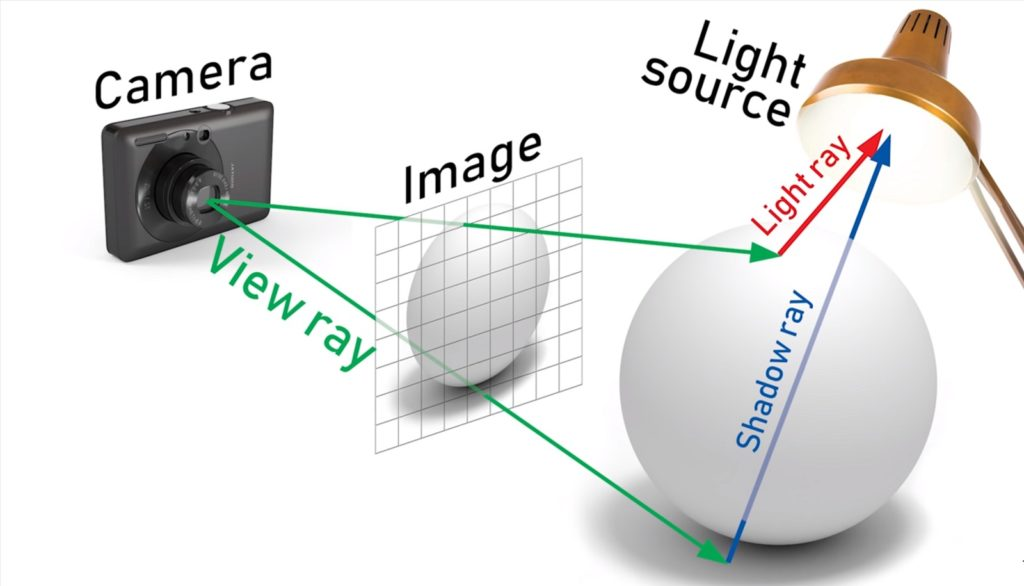
\includegraphics[width=8cm]{images/raytracer_2.jpg}
     \caption{Ray casting illustration, where rays are travelling from the camera/sensor towards the scene. \protect\cite{Kimathi2020}}
        \label{fig:dice}
\end{figure}


Other approaches such as Rasterization can be used to overcome these obstacles; however, Raytracing algorithms can provide more realistic images than Rasterization even though they take more time to render a scene. This is the reason why  Rasterization is used for real-time applications such as gaming more than Raytracing; on the other hand, Raytracing is more often used in offline applications such as simulations and interior design software.
\clearpage

\begin{figure}[h]	
     \centering
     \captionsetup{justification=centering,margin=2cm}
     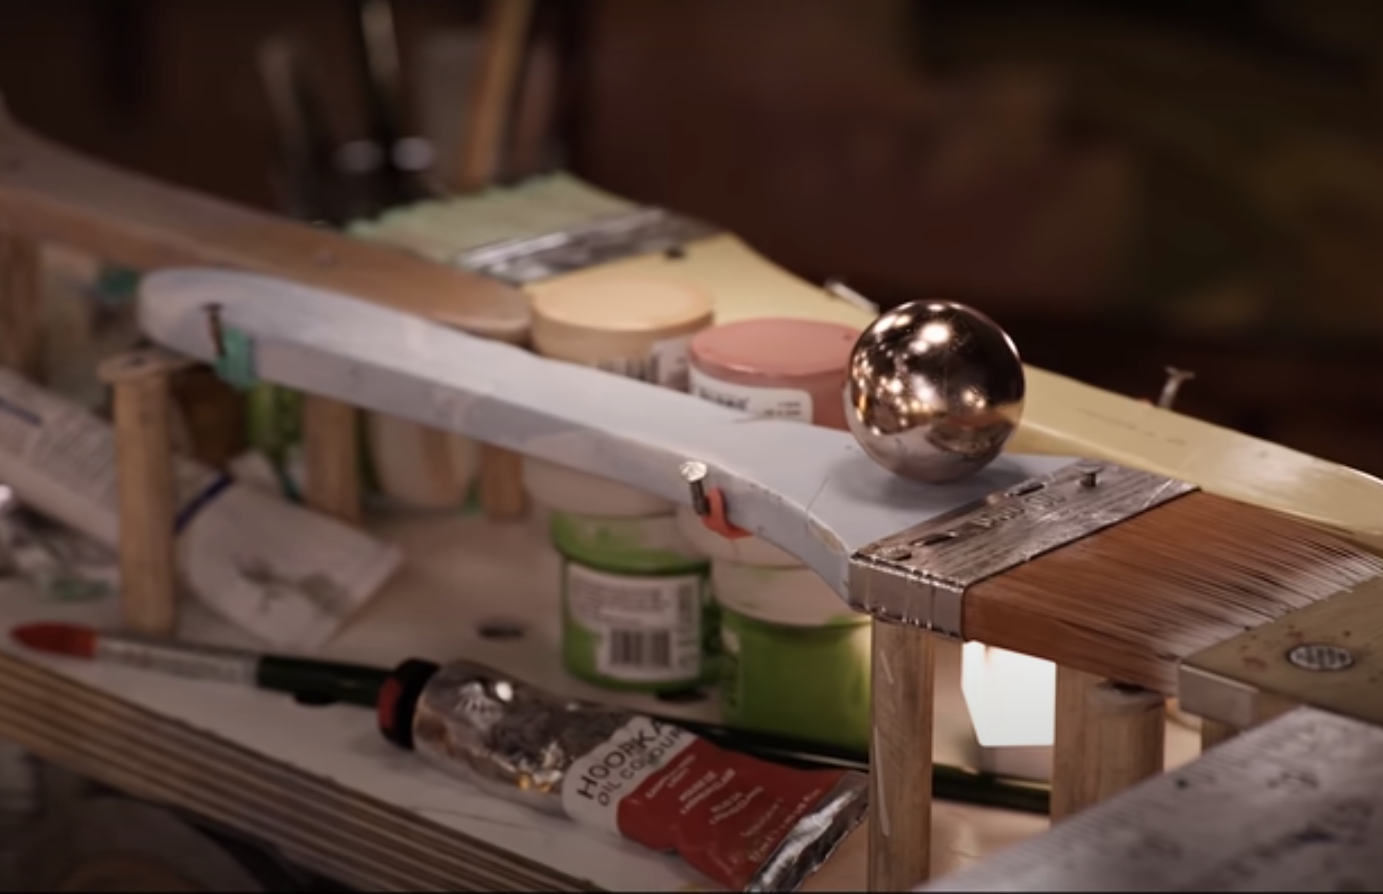
\includegraphics[width=10cm]{images/marbel_brush.png}
     \caption{Marbles RTX playable demo using NVIDIA RTX 3080 Technology to Realizes Dream of Real-Time Cinematic Rendering.\protect\cite{Burke2018}}
        \label{fig:dice}
\end{figure}

In Game Developers Conference - NVIDIA announced NVIDIA RTX™, a ray-tracing technology that brings real-time, cinematic-quality rendering to content creators and game developers. (Brian Burke, 2018), the results where promising and shows that having a real-time raytracer is possiable with the advancement of GPUs. 
\\
\noindent

The lighting and the shadows are so detailed in the scene that they look like a picture taken from a camera and not generated from a computer. The real challenge is real-time raytracers, which require rendering approximately 50 high-quality frames per second.
\\
\noindent

We should understand how challenging to render one frame that consists of thousands of primitives in less than one second. 

\subsection{Motivation of using acceleration data structures}
In the Raytracing pipeline, we mentioned that each ray must execute an intersection test with all the primitive contained in the scene.  This means if we have $N$ number of pixels and $P$ number of primitives, this will produce a complexity of $O(N.P)$, this means even if one pixel only contain a premitive we would have to go to all other pxiels and still test them against all premitives. 
\\
\noindent

Brute forcing complexity is high, increasing linearly with the number of primitives. Moreover, some features such as anti-aliasing require more rays per pixel which increases the complexity to  $O(N.P.S)$ where $S$ is number of samples per pixel. 
\\
\noindent

Using more samples will often produce a higher quality frame; additionally, for better illumination results, more recursion (Shadow rays) must be cast after each intersection. We need more rays but with fewer intersection tests as possible.
\\
\noindent

Let us illustrate this with a simple example, giving a raytracer that uses S: number of samples per pixel = 5, N: number of primitives = 100000, and P: number of pixels =  1280 x 1024, maximum depth = 3. This will give us a number of intersection tests, approximately = 1280 x 1024 x 100000 x 5 x 3 = 1.96608×10¹² intersection test, assuming the machine we are using will spend 0.01ms in each ray. This means for this simple scene the raytracer will render the frame in 220 days. Some scenes contain millions of primitives making, rendering them by brute-forcing imposable. 
\\
\noindent
 
Luckily one can use preprocessing algorithms to reorder and group the primitives to make them quickly tested. Spatial subdivision and object subdivision are the two basic types of data acceleration structures. Spatial subdivision algorithms partition three-dimensional space into areas and keep track of which primitives overlap which regions. On the other hand, object subdivision algorithms gradually subdivide the scene's objects into smaller groups. This way, we can only test the primitives that have a higher probability to intersect with the ray rather than testing all primitives that are not relevant to the region the ray passes through. 

\clearpage

\section{Bounding Volume Hierarchies (BVH)}
\subsection{Concept}
The basic idea of the BVH is simple yet powerful. It is to wrap all primitives in a virtual bounding box. This box will act as metadata to show the limits of the primitive and has no idea of how the shape of the primitive inside it. This concept will make it easier to test the primitives because one can wrap a complex model with one bounding box, and if the ray intersects the bounding box of the model, then and only then can we test its primitives.



\begin{figure}[h]	
     \centering
     \captionsetup{justification=centering,margin=2cm}
     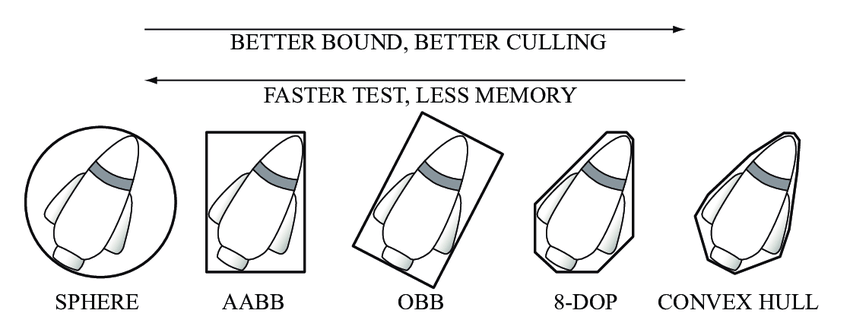
\includegraphics[width=10cm]{images/bvs.png}
     \caption{Bounding volumes: sphere, axis-aligned bounding box (AABB), oriented bounding box (OBB), eight-direction discrete orientation polytope (8-DOP), convex hull . \protect\cite{Ericson2004}}
        \label{fig:dice}
\end{figure}

The bounding box can have different shapes, as shown in Figure. The simpler the bounding box is, the faster and easier to test the intersection. However, the less tightened it becomes and space between the primitive the bounding box boundaries. A compact bounding volume will assist us have the fewest overlaps with other bounding volumes in our scene, while a quick intersection test will help reduce time complexity. In this report, we will be using AABB, because it is easy to implement and easy to test its intersection, and less memory consumption because it only needs to save two double points the minimum and maximum edges of the bounding box. One can use a combination of all of them but in this report we will only use the AABB. 



\begin{figure}[h]	
     \centering
     \captionsetup{justification=centering,margin=2cm}
     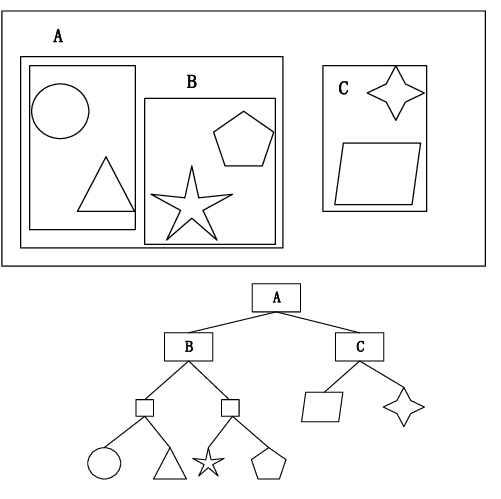
\includegraphics[width=8cm]{images/bvh_tree.png}
     \caption{BVH tree result based on a simple scene. \protect\cite{Ericson2004} }
        \label{fig:dice}
\end{figure}


Let us look at the figure as an example; this scene is consistent of 6 objects. Looking at the generated binary tree, we can note that every two objects are bounded by one AABB, then each two AABB are bounded by a bigger AABB. We recursively do this until we reach the root node that covers the limits of the whole objects. 
\\
\noindent

Without the BVH, we will have to go through all the 6 objects for each ray, even for the rays that do not intersect with any object. On the other hand, when we introduced BVH, we can note that for the rays that do not even intersect with the root AABB node, we do not go further to test its children. This means we will only test once rather than six times. Looking at the sphere, if a ray intersects with it, we will only have to go through a path that goes A -> B -> AABB sphere parent -> Sphere. These are four tests instead of 6. 
\\
\noindent

We know that for a binary tree, the worse case complexity is O(n), but if it is a balanced tree, it becomes O(logn), this is significant, but the catch is we should try to build a balanced binary tree. This is where splitting criteria come in handy. 


\subsection{Implemntation}
BVH has two main implementation pillars, Construction of the BVH tree and Traversal over the tree.  

\subsubsection{Construction}
Before going through the construction details, we have to discuss one essential key in building the BVH tree.  BVH tree comes in different flavors depending on its splitting criteria. Since we are building a tree, the critical question is, when do we split the node? and which axis to choose for splitting? Firstly we will answer the first qquestion. There are three popular strategies to split the node:


\begin{itemize}
\item \textbf{Median of the centroid coordinates (Object median)}:The median of primitives, meaning if we have the next primitive positions in the x-axis as follows ${1, 3, 3, 6, 7, 8, 9}$ the median will be the primitive in the middle, which is $6$. This strategy will produce a well-balanced tree because it splits the primitives into two equal subtrees. Because this method is intuitive to implement and produces a well-balanced tree, this strategy will be adopted in this report. 


\item  \textbf{Mean of centroid coordinates (Object mean)}: Using the man of the premitives going back the example ${1, 3, 3, 6, 7, 8, 9}$, the mean of this set is $5.2$, where the left child node will contain ${1,3,3}$ and the right child ${6,7,8,9}$

\item  \textbf{Spatial median}: Splitting the premitives volume into two equal parts. For example, if we have four spheres with the next radius ${1,1,1,4}$, this strategy will split it as follow, the left child is ${1,1,1}$ and the right child is ${4}$ because it will split based on the volume/area of the sphere and not the position as the previous strategies. 

\end{itemize}


\begin{figure}[H]	
     \centering
     \captionsetup{justification=centering,margin=2cm}
     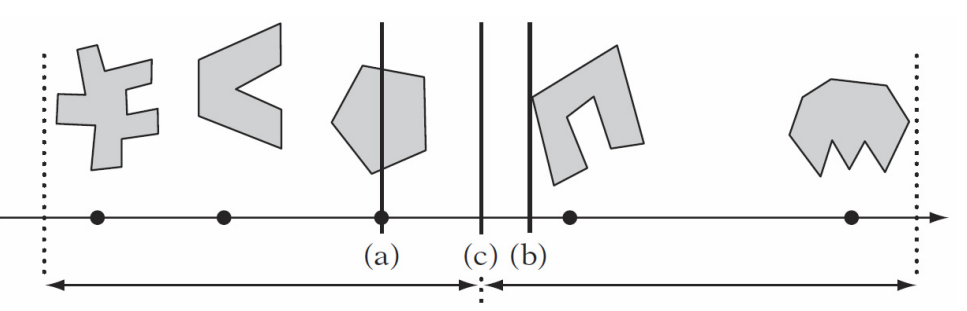
\includegraphics[width=10cm]{images/bvh_split.png}
     \caption{An example of (a) Object median splitting (b) Object mean splitting (c) Spatial median
splitting based on \protect\cite{Ericson2004}}
        \label{fig:dice}
\end{figure}


To answer the second question, which axis to choose for splitting? One can use any axis, but this is a naive way to split. What happens if all primitives have the same z-axis and y-axis, but only the x is changing, and we randomly choose to split by z-axis! This will usually produce an unbalanced tree. The optimal way is to calculate the longest axis for each node (AABB box). This way, we can try to split by the longest axis, which will produce a better-balanced tree. We can find the longest axis of the AABB box by using its diagonal $d$.  

\begin{equation}
\textbf{d} = \textbf{AABB}_{max} - \textbf{AABB}_{min}
\end{equation}

In the Figure, we have four spheres and an AABB covering all the spheres. If we would like to choose one axis to split from, we can randomly start with the x-axis. As it is illustrated, choosing this axis will not give us a middle point to split point since all spheres have the same x-axis. Same for the y-axis. On the other hand, we can see that the Z-axis will split the AABB box into two AABB boxes, each containing two spheres. 

\begin{figure}[H]	
     \centering
     \begin{subfigure}[b]{0.3\textwidth}
         \centering
         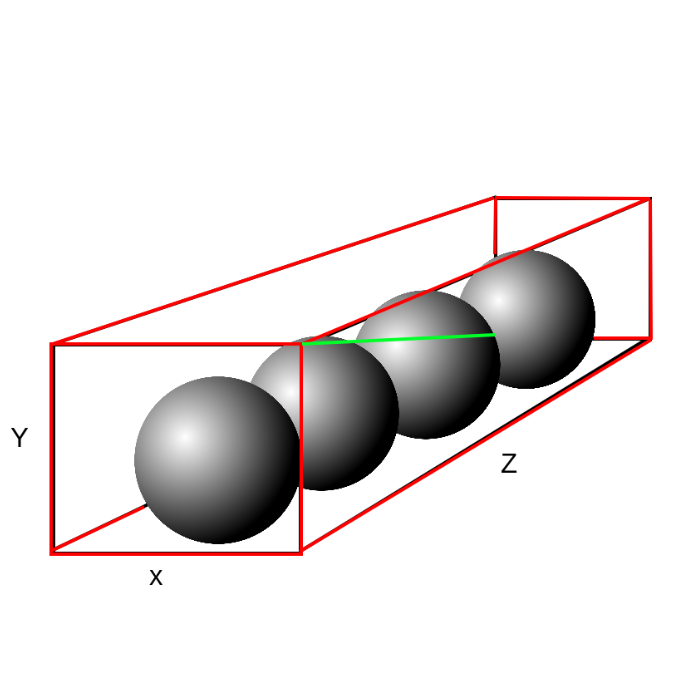
\includegraphics[width=\textwidth]{images/longaxis.png}
         \caption{AABB covers four spheres and its diagonal in green.}
         \label{fig:pi_4000}
     \end{subfigure}
     \hfill
     \begin{subfigure}[b]{0.3\textwidth}
         \centering
         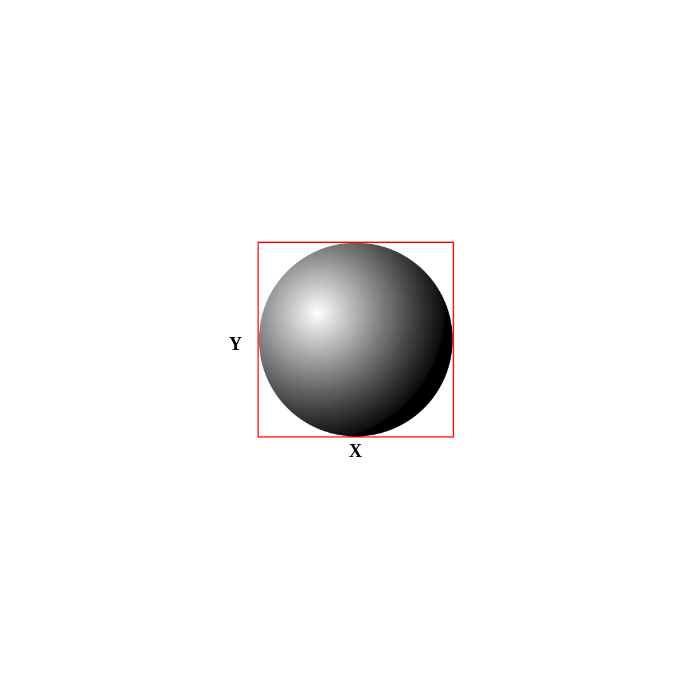
\includegraphics[width=\textwidth]{images/LONGAXIS_Y.png}
         \caption{Finding a split point for x and y axis is not useful for bueling a blaanced tree.}
         \label{fig:pi_5000}
     \end{subfigure}
     \hfill
     \begin{subfigure}[b]{0.3\textwidth}
         \centering
         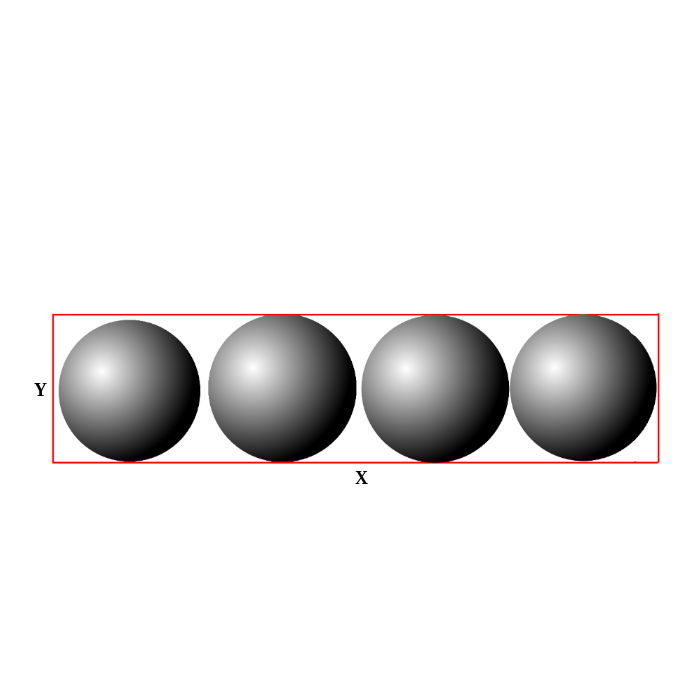
\includegraphics[width=\textwidth]{images/LONGAXIS_Z.png}
         \caption{Z-axis has the best premitives spread that build a balanced tree.}
         \label{fig:pi_18000}
     \end{subfigure}
        \captionsetup{justification=centering,margin=2cm}
        \caption{The scene contains four spheres with the same x-axis and y-axis but different z-axis. }
        \label{fig:three graphs}
\end{figure}

\subsubsection{Visual Illustration}
For a better illustration of how to build the BVH tree by using the Median of the centroid coordinates splitting criteria and also by choosing the longest axis to split from, we will look at the next scene as an example: 

\begin{figure}[h]	
     \centering
     \begin{subfigure}[b]{0.3\textwidth}
         \centering
         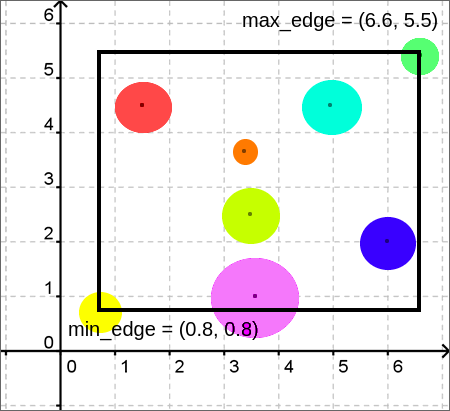
\includegraphics[width=\textwidth]{images/example_bvh/2.png}
         \caption{Root node AABB covers all premitives}
         \label{fig:pi_4000}
     \end{subfigure}
     \hfill
     \begin{subfigure}[b]{0.3\textwidth}
         \centering
         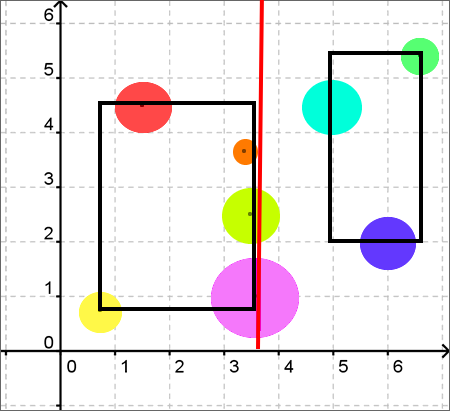
\includegraphics[width=\textwidth]{images/example_bvh/3.png}
         \caption{Second level in the tree splites the prmitives to two groups.}
         \label{fig:pi_5000}
     \end{subfigure}
     \hfill
     \begin{subfigure}[b]{0.3\textwidth}
         \centering
         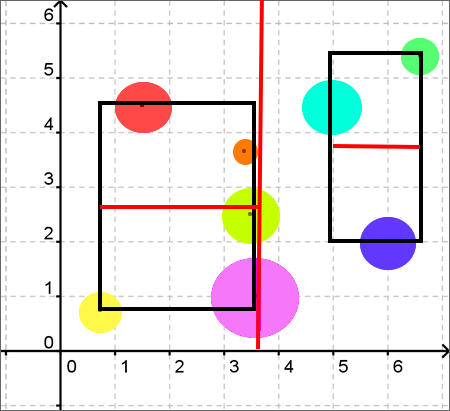
\includegraphics[width=\textwidth]{images/example_bvh/4.png}
         \caption{Last level of the split}
         \label{fig:pi_18000}
     \end{subfigure}
        \caption{Creating AABBs boxes}
        \label{fig:three graphs}
\end{figure}

Firstly, we start creating the root node by calculating the $minimum\_edge$ (the smallest bounding point in our AABB) and the $maximumu\_edge$ point (the largest in the AABB box). This can be easily done by iterating through all primitives and assigning the smallest primitive centroid to the  $minimum\_edge$ and the largest primitive centroid to the $maximum\_edge$.
\\
\noindent

The second step is to split the primitives in the node by using the AABB boundaries. As we mentioned, we will find the longest axis.
To find the longest axis, we subtract the $minimum\_edge$ from $maximum\_edge $ and find the maximum of both axes $max(maximum\_edge - minimum\_edge)$. This will give us $max((6.6-0.8) - (5.5-0.8)) = max(5.8,4.7) = 5.8$, which is the x-axis. 
\\
\noindent

Now we calculate the splitting point by just halfing the distance between $maximum\_edge $ and the $minimum\_edge$, $split\_point\_x = (0.8+6.6) / 2 = 3.6$.
\\
\noindent

We then create a left node that contains the primitives less than 3.6 and a right node that contains the primitives with a centroid $ > 3.6$. 
\\
\noindent

Recustivly we keep doing this until we reach a $maximum\_leafs$ parameter which is predefined, and in this report, it is $1$. This means the leaf node will only hold one primitive. 


\begin{figure}[h]	
     \centering
     \captionsetup{justification=centering,margin=2cm}
     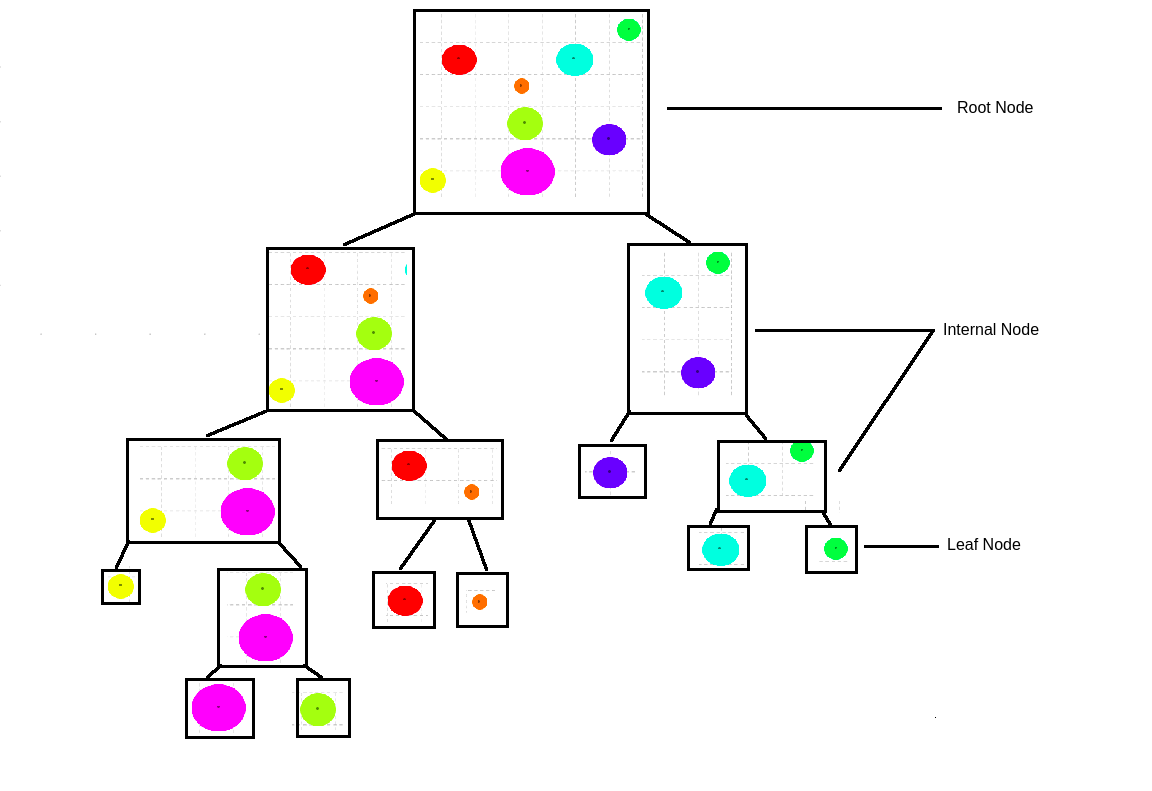
\includegraphics[width=9cm]{images/example_bvh/tree.png}
     \caption{BVH Tree example by using the median split criteria}
     \label{fig:dice}
\end{figure}
\clearpage


\subsubsection{Traversal}
 The traversal phase of BVH is quite intuitive if you are familiar with how binary tree traversal works. After building the BVH tree, we start with its root node, which has the maximum and minimum boundaries of the biggest AABB that bounds the whole scene. We test if the ray intersects the AABB of the root node. If it is true, we go to its left and right children and do the same process; otherwise, we terminate. Recursively keep doing this until we reach the leaf node; the leaf node is the node that has no children, and it is the only node that contains a primitive inside it. Then we go through the list of primitives and test each one if it is intersected with the ray or not. 
\\
\noindent

As discussed, the leaf node can include a list of primitives and not only one by setting a parameter called $max\_leaf\_premitives$ to 1; this depends on how you configure the BVH building tree method. In this report, I set the list to make it only contain one primitive. It is worth noticing that the bigger $max\_leaf\_premitives$ is, the smaller the depth of the tree becomes because we do not have to keep splitting until we reach a leaf that only contains primitives less or equal to $max\_leaf\_premitives$, hence less traversal time and less memory consumption because of the number of nodes saved, on the other having a long list of primitives inside the leaf node is bad for the performance because this will get us to the same challenge we would like to solve by introducing the BVH which is avoiding brute force algorithms.
\\
\noindent

The intersection test is split into two main steps. First, we go through all the nodes in the tree, and if we hit a leaf node, we add all its primitives into a list called $hitList$. Afterward, we go through these candidates and find which are intersected and which one is the closest. The following two pseudo-codes explain the intersection test for the BVH. 


\begin{algorithm}[H]
	\caption{$BVHIntersect$}\label{alg:alg1}
	\begin{algorithmic}
		\Require $ray$, $node$, $hitList$
		\If{$node$ $\rightarrow$ $boxIntersect(ray) = false $}
			\State $return\;\;false$
		\EndIf
		\If{$root$ $\rightarrow$ $isleaf$}
		    \State $hitList$ $\rightarrow$ $push(node \rightarrow premitives)$
		\Else
			\State $BVHIntersect(ray, node \rightarrow leftChild,\, hitList)$
			\State $BVHIntersect(ray, node \rightarrow rightChild,\, hitList)$
		\EndIf
	\end{algorithmic}
\end{algorithm}

\clearpage

\section{Linear Bounding Volume Hierarchies (LBVH)}
\subsection{Concept}
While BVH boosts the renderer's performance and makes it possible to render millions of primitives in minutes, it introduces an extra step in the rendering pipeline, which is a preprocess for building the tree. The building tree process can take half of the rendering time; nevertheless, creating this tree will make the render faster to find the intersected primitive. The question now is, can we do something about it? 
\\
\noindent

One way to solve this is to parallelize this process. This can be done if the subtrees are independent of each other. This is what Linear Bounding Volume Hierarchies do.
\\
\noindent

The first step is to transform the building tree problem into a sorting problem. We map the 3D centroid points for each primitive to one value that can be sorted. Morton codes do this mapping. Morton code map multidimensional data to one dimension while preserving locality of the data points.[WIKIPEDIA]. The transformation is done by interleaving the bits of the premitive centroides in base 2. for example taking a 3D point (x,y,z) the result mortone code will be 

\begin{equation}
 ...z_3y_3x_3z_2y_2x_2z_1y_1x_1z_0y_0x_0
\end{equation}


\begin{figure}[h]	
     \centering
     \captionsetup{justification=centering,margin=2cm}
     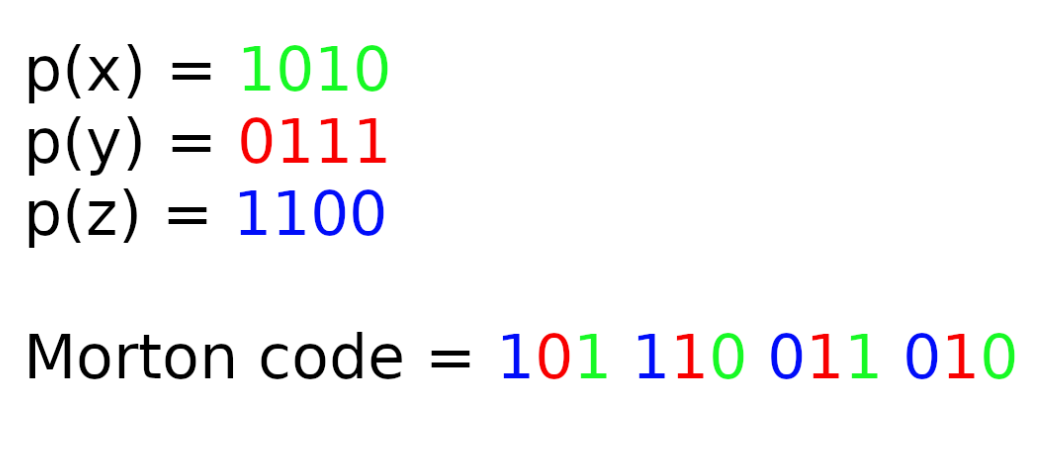
\includegraphics[width=9cm]{images/z_curve.png}
     \caption{Example of mapping a 3D point to a morton code.}
     \label{fig:dice}
\end{figure}


After mapping the 3D point to one 1D Morton code, we can use a sorting algorithm as a Radix sort.

\subsubsection{Visual Illustration}
To better understand how the LBVH constructs the binary tree, we will illustrate this with a scene as shown in Figure. The scene is made out of 16 primitives. The first step is to generate the Morton code for each centroid point. Looking closely into the generated Morton codes of each primitive, we can note that each bit acts as a splitting plane that splits the primitives into more than one region. 
\\
\noindent

The first bit will split the y-axis into two regions. The first region with the first bit equals 1, and the second region with the first bit equals 0. The second bit will split the scene into two areas by an x-axis plane. The third bit will split the y-axis into four regions.


\begin{figure}[H]	
     \centering
     \begin{subfigure}[b]{0.475\textwidth}
         \centering
         \captionsetup{justification=centering}
         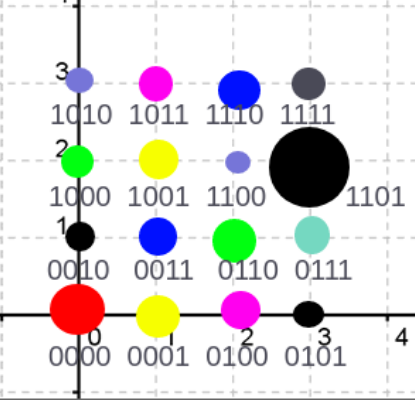
\includegraphics[width=5cm]{images/example_lbvh/scene_2.png}
         \caption{Morton value for premitives center}
         \label{fig:pi_4000}
     \end{subfigure}
     \hfill
     \begin{subfigure}[b]{0.475\textwidth}
         \centering
         \captionsetup{justification=centering}
         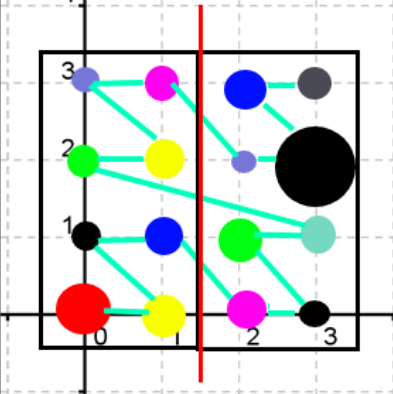
\includegraphics[width=5cm]{images/example_lbvh/02.png}
         \caption{First split on x-axis}
         \label{fig:pi_5000}
     \end{subfigure}
     \hfill
     \begin{subfigure}[b]{0.475\textwidth}
         \centering
         \captionsetup{justification=centering}
         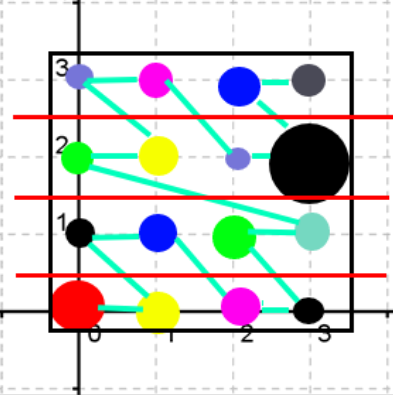
\includegraphics[width=5cm]{images/example_lbvh/03.png}
         \caption{Second split on y-axis}
         \label{fig:pi_18000}
     \end{subfigure}
        \captionsetup{justification=centering,margin=2cm}
             \hfill
     \begin{subfigure}[b]{0.475\textwidth}
         \centering
         \captionsetup{justification=centering}
         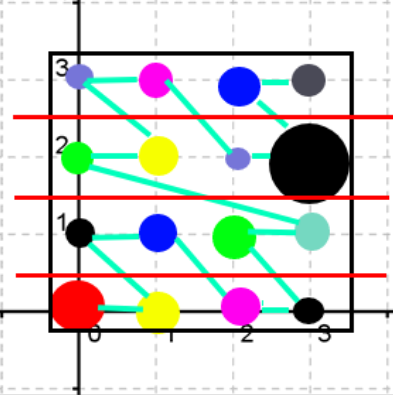
\includegraphics[width=5cm]{images/example_lbvh/03.png}
         \caption{Third split on x-axis}
         \label{fig:pi_18000}
     \end{subfigure}
        \captionsetup{justification=centering,margin=2cm}

        \caption{(a) In 2D, the high bit of the Morton-coded value of a point’s coordinates defines a splitting plane along the middle of the y-axis. If the high bit is set, the point is above the plane. (b) Similarly, the second-highest bit of the Morton value splits the x-axis in the middle. (c) If the high y bit is 1 and the high x bit is 0, the point must lie in the shaded region. (d) The second-from-highest y bit splits the y axis into four areas. }
        \label{fig:three graphs}
\end{figure}



\begin{figure}[h]	
     \centering
     \captionsetup{justification=centering,margin=2cm}
     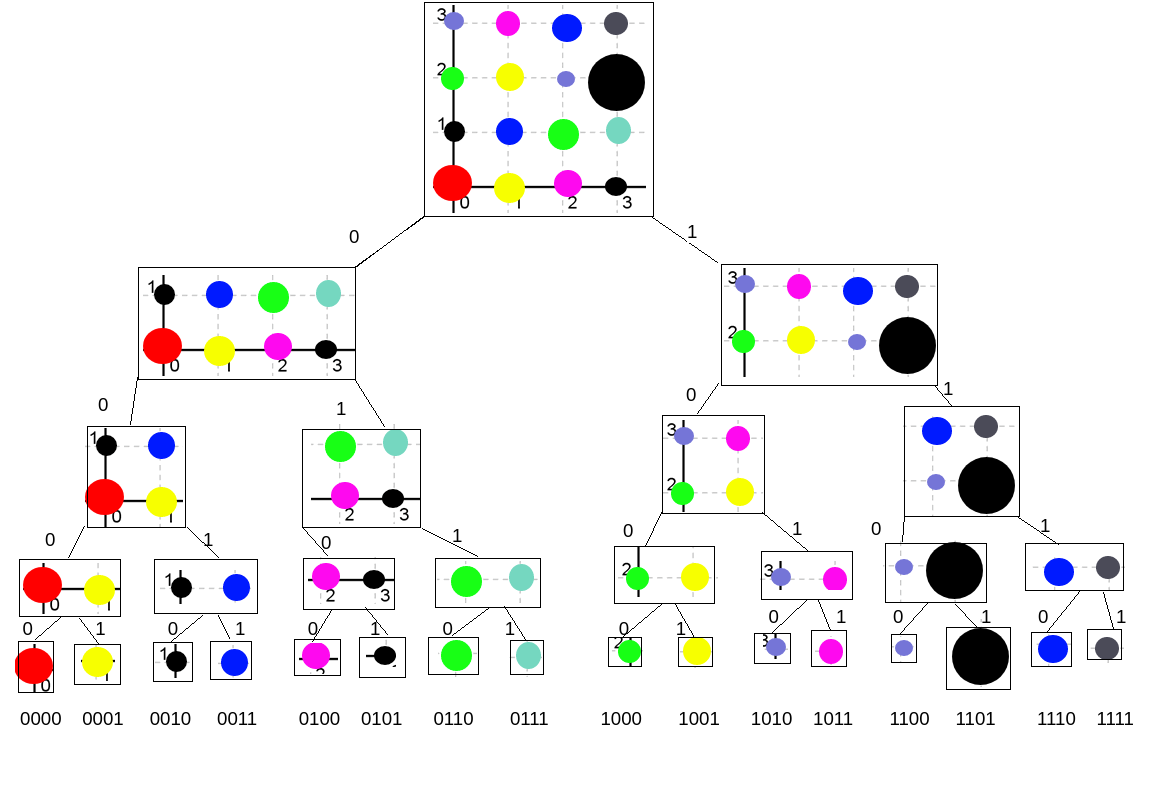
\includegraphics[width=10cm]{images/example_lbvh/tree.png}
     \caption{Generated tree by LBVH.}
     \label{fig:dice}
\end{figure}


\subsection{Implemntation}
The implementation can be done in two main steps, building the tree and tree traversal. Traversal will not be repeated since the produced tree is a binary tree similar to the BVH. Hence the same traversal algorithm used in the BVH will be utilized for LBVH. But the main focus of the LBVH is building the tree.


\subsubsection{Construction}
 Building the tree needs to calculate the Morton code for each primitive. There are two methods for generating Morton code, magic bits, and a lookup table. We will use the magic bits method. After generating the Morton code for each primitive, we will use the Radix sort.
\\
\noindent

Next step to building the tree, we would like to find the splitting point. As we discussed before, LBVH splits the space into two regions based on the first-bit difference. This means the leftChild will contain all primitives with a Morton code with a first bit equal to 0, and the rightChild will contain the primitives with Morton codes with a first bit equal to 1. Since the Radix sort already sorts the primitives, we can do the splitting by simply using an Exponential search. 
\\
\noindent

We start with a random split point. Let us say the last points. Then we start decreasing exponentially to search for the first bit differing from 0 to 1. One way to check this is to use some bit operations; however, another approach is to count the number of leading zeros and compare them with the previous one. If they differ, then we can split. 
\\
\noindent

Until this point, we are not gaining much if using LBVH. As we discussed, LBVH special is how easily we can parallelize it. To achieve this, we will use a simple conditional multithreading mechanism. For building the tree we will only create a new thread of the number of premitives in the subtree is more than 100 premiitive. Note that this is a random number chosen, but we do not want to create a new thread for small subtrees because it is not worth it anyway.

\begin{algorithm}[H]
\caption{Pseudocode of the method $LBVH\_construct$}\label{alg:alg1}
\begin{algorithmic}
\Function {ConstructLBVH}{$allSceneObjects$, $sortedMortonCodes$, $sortedMortonCodes$, $startIndex$, $endIndex$, $totalNodes$ }
\State $totalNodes++$
\State $node \gets Node()$
\State $aabbBoundries \gets findBiggestAABBBoundries(allSceneObjects)$
\State $objectsNumber \gets  endIndex - startIndex$
\If{$objectsNumber = 0$}
	\State $node \rightarrow isleaf \gets true$
	\State $node \rightarrow objs \gets allSceneObjects[startIndex]$
	\State \Return $node$
\EndIf

\State $midPoint \gets findSplitPoint(sortedMortonCodes, startIndex, endIndex)$
\State $node \rightarrow leftchild  \gets constructBVHNew(allSceneObjects, startIndex, midSplitIndex, totalNodes)$
\State $node \rightarrow rightchild  \gets constructBVH(allSceneObjects, midSplitIndex, endIndex, totalNodes)$
\State \Return $node$
\EndFunction
\end{algorithmic}
\end{algorithm}
\clearpage



\section{K dimensional tree (Kd-Tree)}
\subsection{Concept}
We have already covered two data structures accelerators, the BVH and LBVH. Both methods are under the category of object subdivision. This chapter will discuss and implement a different accelerator called KD-Tree.
KD-tree is a traditional data structure that organizes K-dimensional points into a binary tree for easy retrieval. The KD tree can have several dimensions at each level, unlike a typical binary tree. It has been frequently utilized in multidimensional crucial data search because of its effective performance in resolving multidimensional searching issues.
\\
\noindent

Unlike the previous techniques, KD-Tree is a method categorized as a space subdivision.
Space subdivision algorithms split the space into areas and assign the primitives that fall in those areas.
\\
\noindent

The main idea is to divide the scene into regions. Each region will have a list of primitives that intersect it. When we start rendering and start the intersection tests, we start looking for areas that intersect with the ray, and if we find an intersection, we only test the primitives that fall in it.
The following figure gives an overview of how the spaces are divided: 

\begin{figure}[h]	
     \centering
     \captionsetup{justification=centering,margin=2cm}
     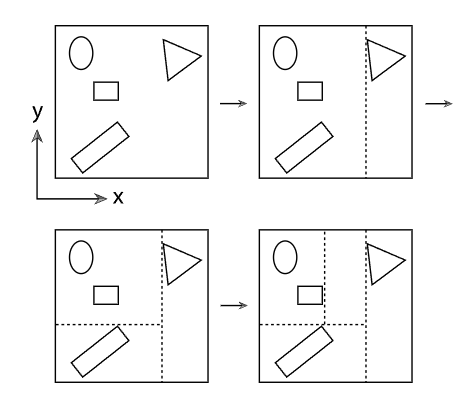
\includegraphics[width=10cm]{images/kdtree/example_demo.png}
     \caption{The Kd-tree is built by splitting the scene into four regions where in each node one axis is chosen with a splitting point.  The first split is done on the x-axis then y and the last split is on the x-axis again. The refinement criteria's specifics, such as which axis is used to partition space at each stage, where the plane is positioned along the axis, and when refinement ends, can have a significant impact on how well the tree performs in actual use. \protect\cite{Pharr2016}}
        \label{fig:dice}
\end{figure}



\subsubsection{Compact tree representation}
Unlike what we did in the BVH, the representation of the tree will be compact. This means rather than saving two children pointers left and right, we will save all nodes in an array, where the left child lives right after the parent node in the array, and the right child can be reached by saving the offset. Doing so improves cache, memory, and thus overall system performance.


\begin{figure}[h]	
     \centering
     \captionsetup{justification=centering,margin=2cm}
     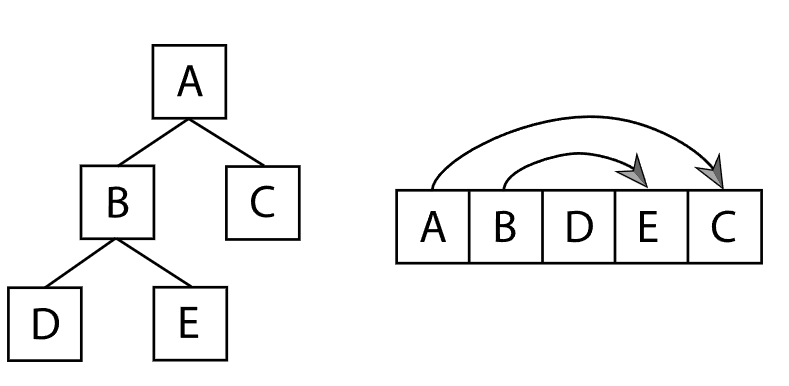
\includegraphics[width=8cm]{images/kdtree/compact.png}
     \caption{Linear Layout of a KD-Tree in Memory. The  first child is discovered immediately after the parent node in memory. An offset pointer, illustrated here with lines and arrows, is used to locate the second child. The tree's leaf nodes (D, E, and C) have no children.\protect\cite{Pharr2016}}
        \label{fig:dice}
\end{figure}


\subsubsection{The Surface Area Heuristic}
Though there are several methods for creating BVHs and kd-trees, the most well-known method for increasing traversal efficiency for both data structures is to use a top-down, greedy surface area heuristics (SAH) build, in which the original scene is recursively partitioned using a greedy strategy for minimizing expected traversal cost. 
\\
\noindent

Given a collection of N primitives in a sub-tree that spans the 3D volume V, and assuming that the sub-tree is partitioned into two halves L and R with number of triangles NL and NR, and corresponding volumes VL and VR, respectively, the projected traversal cost may be approximated as

\begin{equation}
Cost(V) = C_T + C_I(\frac{SA(V_L)}{SA(V)}N_L \frac{SA(V_R)}{SA(V)}N_R)
\end{equation}

Where: $V$: Volume, $C_T$: Cost of traversal, $C_I$: Cost of intersection, $SA$: Surface area, $N$: Number of premitives, $•L$: Left, $R$: Right.
\\
\noindent

Let us have an exmaple for betrter vudal illustration on how the SAH works: 

Giving the next scene consists of 7 primitives, we would like to find the best split by using the SAH method. Because the intersection cost depends on the raytracer implementation and also varies between the different shapes of primitives, for easier calculation, we will set it to 1. In contrast, while the estimated traversal cost was set to $\frac{1}{8}$. We will set the number of buckets to 8.
\\
\noindent

Starting with the first iteration, the green is the left area, and the red area is the right. Since the example is in 2D, the SA equals the width x height of the square. Each pixel has an area of 1. The SA of each square is illustrated in the figure. The overall surface area SA equals to the summation of all the 7 prmitives $1+1+4+4+4+1+1 = 16$ We can now substitute all the given information into the equation we get: 


\begin{equation}
Cost\_iteration\_1 =  \frac{1}{8} + (\frac{1}{16}(1) +\frac{1+4+4+4+1+1}{16}(6)) = 5.81
\end{equation}

\begin{equation}
Cost\_iteration\_2 =  \frac{1}{8} + (\frac{1+1}{16}(2) +\frac{4+4+4+1+1}{16}(5)) = 4.75
\end{equation}

\begin{equation}
Cost\_iteration\_4 =  \frac{1}{8} + (\frac{1+1+4}{16}(3) +\frac{4+4+1+1}{16}(4)) = 3.75
\end{equation}

\begin{equation}
Cost\_iteration\_7 =  \frac{1}{8} + (\frac{1+1+4+4+4+1}{16}(6) +\frac{1}{16}(1)) = 5.81
\end{equation}


We choose the minimum cost. In the previous iterations, it is the 4th and then assigns the primitives on the left to the left node and the right primitives to the right node. Unlike BVH, some primitives can be set to both left and right if they are between the bucket's splitting point.


\begin{figure}[H]	
     \centering
     \begin{subfigure}[b]{0.475\textwidth}
         \centering
         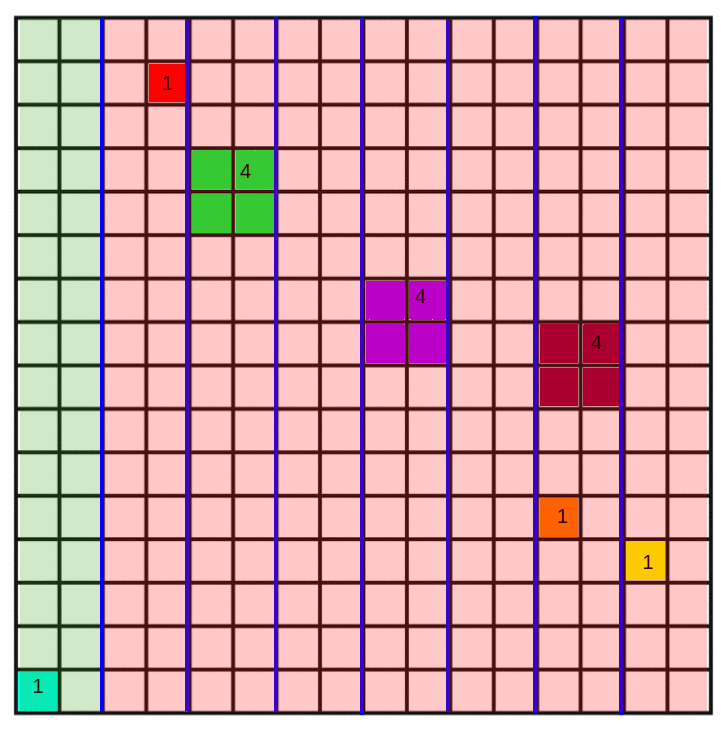
\includegraphics[width=5cm]{images/kdtree/grid_2.png}
         \caption{$1^{st} $ iteration.}
         \label{fig:pi_4000}
     \end{subfigure}
     \hfill
     \begin{subfigure}[b]{0.475\textwidth}
         \centering
         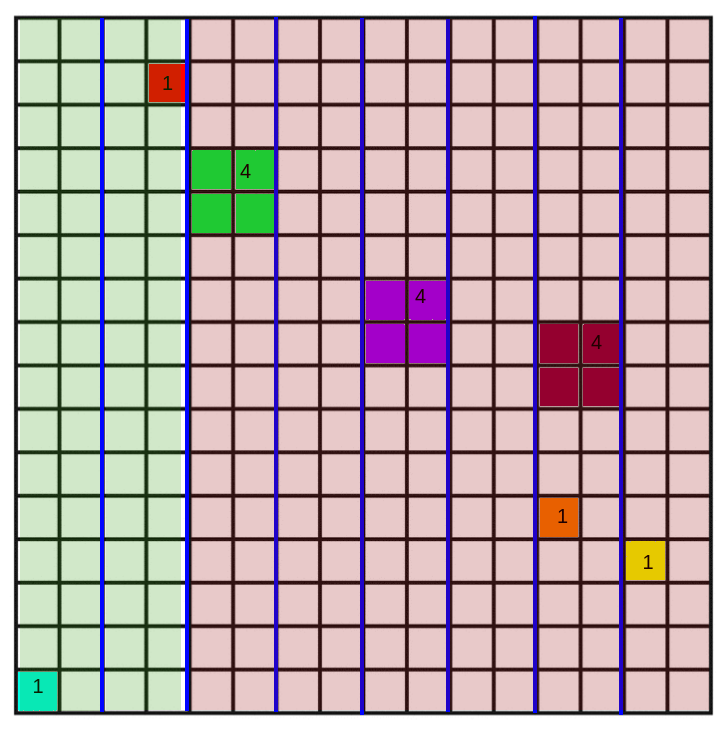
\includegraphics[width=5cm]{images/kdtree/grid_3.png}
         \caption{$2^{nd} $ iteration.}
         \label{fig:pi_5000}
     \end{subfigure}
     \hfill
     \begin{subfigure}[b]{0.475\textwidth}
         \centering
         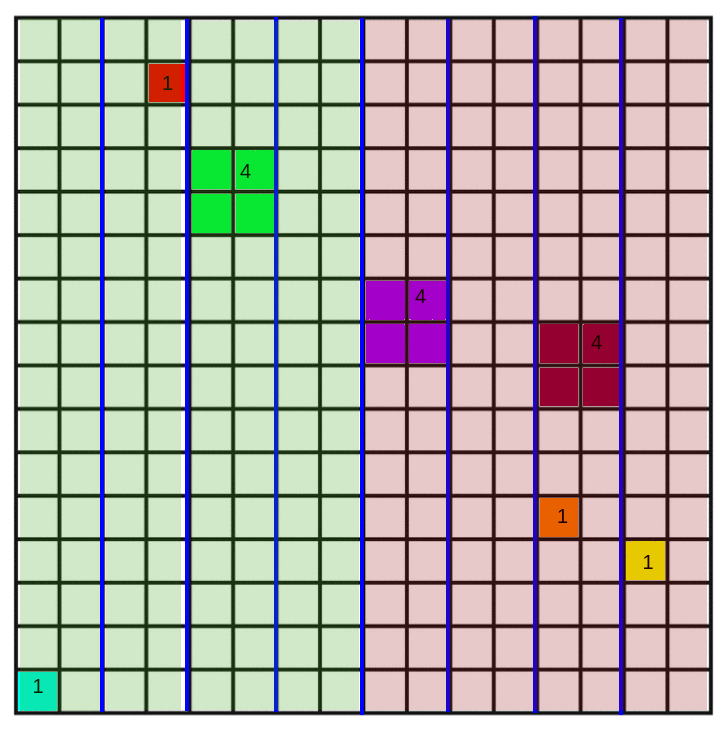
\includegraphics[width=5cm]{images/kdtree/grid_5.png}
         \caption{$4^{th} $ iteration.}
         \label{fig:pi_18000}
     \end{subfigure}
     \hfill
     \begin{subfigure}[b]{0.475\textwidth}
         \centering
         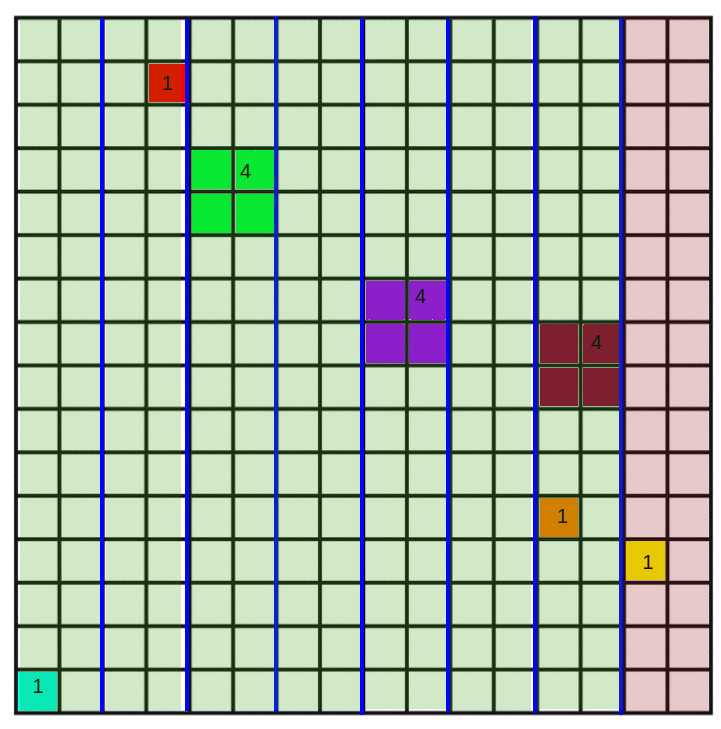
\includegraphics[width=5cm]{images/kdtree/grid_8.png}
         \caption{$7^{th} $ iteration.}
         \label{fig:pi_18000}
     \end{subfigure}
        \captionsetup{justification=centering,margin=2cm}
        \caption{Visual illustration of the different left (green) and right (red) regions for calculating the SAH cost to find the best splitting point. }
        \label{fig:three graphs}
\end{figure}



\subsection{Implemntation}

Kd-Tree is a variant of Binary space partitioning (BSP) tree. BSP trees use planes to divide the space into regions. It follows a top-down approach where a bounding box bounds the whole scene. If the number of primitives inside the bounding box exceeds a pre-defined parameter, we will name it maxPrims then, the box is split into two sub-regions based on chosen splitting criteria. Each primitive is associated with the corresponding box/region that it intersects with. This means duplicated primitives that can live in more than one box, unlike the BVH.
\\
\noindent

The procedure keeps repeating recursively until one of the two ending conditions occurs. Either the number of primitives in the sub-regions is less than maxPrims or the other parameter, maxdepth is reached. maxdepth parameter is used to control the depth of the tree. 
\\
\noindent

In order to increase the efficiency of traversal and tree construction, kd-trees simply limit the splitting plane to only be perpendicular to one of the coordinate axes. However, this compromises some flexibility in how space is divided.

\subsubsection{Construction}

The recursive top-down algorithm is used to construct the kd-tree. We have a collection of primitives that overlap the axis-aligned space region at each step. Either the region is divided into two smaller ones and transformed into an inner node, or the recursion is stopped by making a leaf node out of the overlapping primitives.
\\
\noindent

In the Kd-tree, we will save the nodes in an array and not in a tree representation, as mentioned before, increasing caching. The issue is how to predetermine the number of nodes before building the tree to initiate the array? There are two approaches here. The first is to build the binary tree and then flatten it to an array (compact representation). The second approach is to allocate memory as we build the tree dynamically. The first approach needs two steps to build the tree and then transform it into a compact form, adding an extra step that reduces performance. Also, it consumes more memory as it eeds to save the tree and adds an array that contains the same number of nodes as the tree. The second approach is preferred as it consumes less memory and improves performance. However, it needs better handling for the memory allocation, this complexity depends on the implmentation and the programming language is used, so I will not explain the implementation. 
\\
\noindent

For building the tree, the maximum allowed depth is needed to be given. However, what depth is preferred, large or too small? Large depth will increase the number of nodes, increasing memory consumption. Reducing it will reduce the number of nodes but will make the traversal time more linear, killing the use of the binary tree to reduce the complexity. Based on  PBRT book, a generic formula can be used to calculate the depth. This formula works for a various scenes, $N$ is the number of primitives in the scene. 


\begin{equation}
depth = 8 + 1.3log(N)
\end{equation}


Since we are using memory allocation dynamically for the nodes array, each time the array is full, we will then reallocate more memory duoble the size of the old array.
\\
\noindent

The splitting point will be found using the SAH algorithm, unlike in the BVH where we used the median point. The advantage of using median point is intuitive to calculate and implement; nevertheless, it does not care about the area/volume of the primitive, unlike SAH, which considers the area/volume. Two parameters $t_{isect}$ and $t_{t_trav}$ are used in the SAH that will be tested and tweaked to find the best parameters. There are different methods to search for the best parameters for the best scenes; nevertheless, we will focus on the ratio between the two parameters instead. PBRT suggests to used 80 and 1, respectively, and other references suggest that the values should stay closer to each other. 
\\
\noindent

One extra parameter, "emptyBonus" denoted as $b_e$ will be added to the SAH algorithm. Since rays traveling through empty areas can progress to the next kd-tree node without having to do any ray-primitive intersection checks, hence there is a little advantage for picking splits when one of the children has no primitives overlapping it. The parameter takes a value between 0 and 1 if one of the regions is empty and 0 otherwise. 

\begin{equation}
Cost(V) = C_T + (1-b_e)C_I(\frac{SA(V_L)}{SA(V)}N_L \frac{SA(V_R)}{SA(V)}N_R)
\end{equation}

One challenge left, if we want to consider all the splitting points as candidates, computing the cost of splitting is expensive, but as we mentioned before, we can use a fixed number of buckets. However, which is the best number for this parameter? The bigger the number, the more accurate the splitting point will be at the cost of building the tree's performance because more calculations are needed. Instead of considering splits at intermediate points, the minimal cost will be reached at a split that coincides with one of the faces of one of the bounding boxes of the primitive. Hence we will need at each cost calculation at most $2 * N$ where $N$ is the number of primitives.

\begin{figure}[H]	
     \centering
     \captionsetup{justification=centering,margin=2cm}
     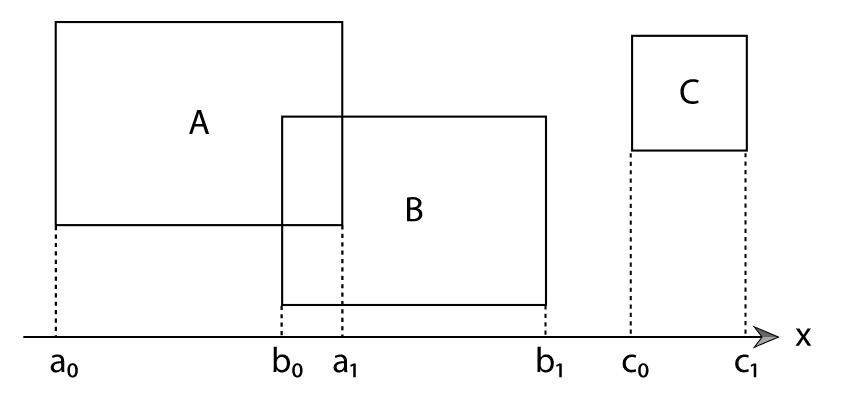
\includegraphics[width=10cm]{images/kdtree/projected_bboxes.png}
     \caption{Only six splitting points are considered. Taking $a_1$ as the splitting point will leave a bounding box under it, B overlapping it, and C above it. \protect\cite{Pharr2016}}
        \label{fig:dice}
\end{figure}

Some edge cases can occur when the same number of primitives are assigned for both children. At this point, we are not gaining any performance from creating an interior node. The solution is to try other axes instead of the best-chosen axis. If the same edge case occurred for all axes, we would create one leaf node and assign all the primitives. It also can be worse to split than creating a leaf node based on the SAH algorithm. In that case, a leaf node is created rather than splitting. 
\\
\noindent

The KD-Tree has a variety of implementations, the one used in this project is based on (Physically Based Rendering). The implementation generates a binary tree that focuses on less memory consumption and finds the best split by using the SAH method for splitting. We will be using a top-down approach as we did in BVH. We will split the implementation into two phases: Tree construction and tree traversal.



\begin{algorithm}[H]
\caption{Pseudocode of the method $buildTree$}\label{alg:alg1}
\begin{algorithmic}
\Function {BuildTree}{$nodeNum$,
	$nodeBounds$,
	$allPrimBounds$,
	$primNums$,
	$nPrimitives$,
	$depth$,
	$edges[3]$,
	$prims0$,
	$prims1$,
	$badRefines$, 
	$primitiveIndices$
 }
\State $totalNodes++$
\If{$nPrimitives  \leq maxPrims || depth == 0$}
	\State $nodes[nodeNum] \rightarrow push \gets InitLeaf(primNums, nPrimitives, primitiveIndices)$
	\State \Return
\EndIf

\State $splitAxis \gets GeMaximumAxis(nodeBounds)$
\State $splitPoint \gets findBestSplitPointBySAH(splitAxis)$
\State $setNodeBoundries(node)$
\State $nodes[nodeNum] \rightarrow push \gets InitInterior(splitAxis, aboveChild, splitPoint)$

\State $buildTree(nodeNum+1, bounds0, allPrimBounds, prims0, n0, depth - 1, edges, prims0, prims1 + nPrimitives, badRefines, primitiveIndices)$

\State $buildTree(aboveChild, bounds1, allPrimBounds, prims1, n1, depth - 1, edges, prims0, prims1 + nPrimitives, badRefines, primitiveIndices)$

\EndFunction
\end{algorithmic}
\end{algorithm}

\subsubsection{Traversal}
The kd tree traversal is different from the BVH traversal we mentioned. BVH was a binary tree traversal where we start with the root node and go to the left or right child. On the other hand, the Kd-tree uses the compact form array. 


\begin{figure}[H]	
     \centering
     \captionsetup{justification=centering,margin=2cm}
     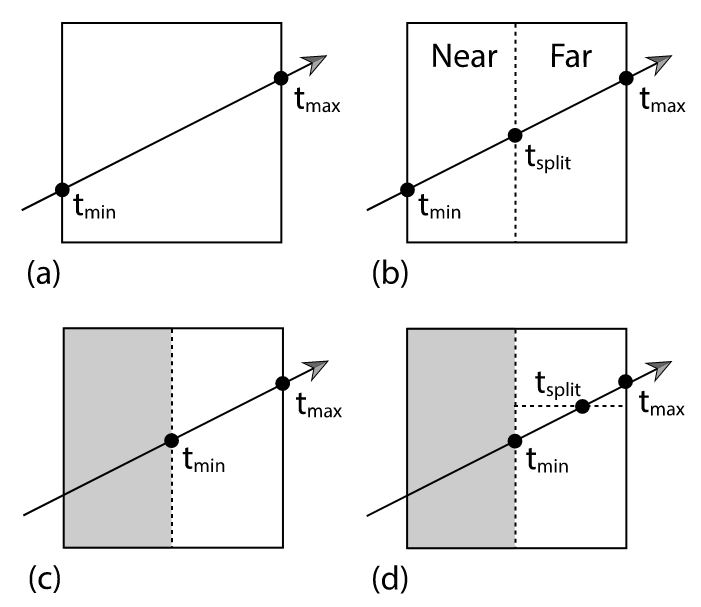
\includegraphics[width=10cm]{images/kdtree/traversal.png}
     \caption{(a) The ray is intersected with the bounds of the tree, giving an initial parametric $[t_{min}, t_{max}]$ range to consider. (b) Because this range is nonempty, it is necessary to consider the two children of the root node here. The ray first enters the child on the right, labeled “near,” where it has a parametric range $[t_{min}, t_{split}]$. If the near node is a leaf with primitives in it, ray–primitive intersection tests are performed; otherwise, its children nodes are processed. (c) If no hit is found in the node, or if a hit is found beyond $[t_{min}, t_{split}]$, then the far node, on the left, is processed. (d) This sequence continues—processing tree nodes in a depth-first, front-to-back traversal—until the closest intersection is found or the ray exits the tree. \protect\cite{Pharr2016}}
        \label{fig:dice}
\end{figure}


The first intersection test will start by testing if the ray intersects the global bounding box of the whole kd-tree $[t_{min}, t_{max}]$. If it returns false, we stop testing other nodes in the tree instantly because this means the ray does not pass any primitive.
\\
\noindent

If it returns true, we proceed to the next step, if the current node is a leaf or an interior node. If it is a leaf node, we iterate through the list of the primitives assigned to the node. As we discussed, we are not saving the primitives directly in the leaf node. We only save the number of primitives and the offset of the indices. This is a huge performance advantage, especially for the kd-tree, because in the kd-tree, one primitive can be in more than one node at a time. In terms of memory usage, if one leaf contains an N number of primitives, then there is a high chance of duplication of information with another leaf that contains these N primitives. You can imagine with a million primitives. This can be at least twice the number of the original primitives. Since we are using a depth-first search, if we reach the leaf node, we will decrement the node index to go back one step, then we reassign the current node and its tMin and tMax values. Note that before going through all the primitives, if the ray already intersected primitives in other nodes and those other nodes and the intersected point is less than the $t_{min}$ of the current node, then we are sure that we can not do better. We will not find any closer primitive in the leaf node. Hence we break and return. 
\\
\noindent


Otherwise, if it is an interior node, we would like to test its children, and unlike we did in the BVH we were going left and then right. This time we will use the intersection point to determine which is the left and the right node. By comparing the splitting point with the intersected point, we can determine which of the children has a higher chance of being intersected first. This can be done quickly by checking if $t_{split} > t_{max}$, then we do not need to check the far child node, same we check if $t_{split} < t_{min}$, then we do not check the far child node. Otherwise, we check them both by starting with the near and proceeding to the far. 

\begin{figure}[H]	
     \centering
     \captionsetup{justification=centering,margin=2cm}
     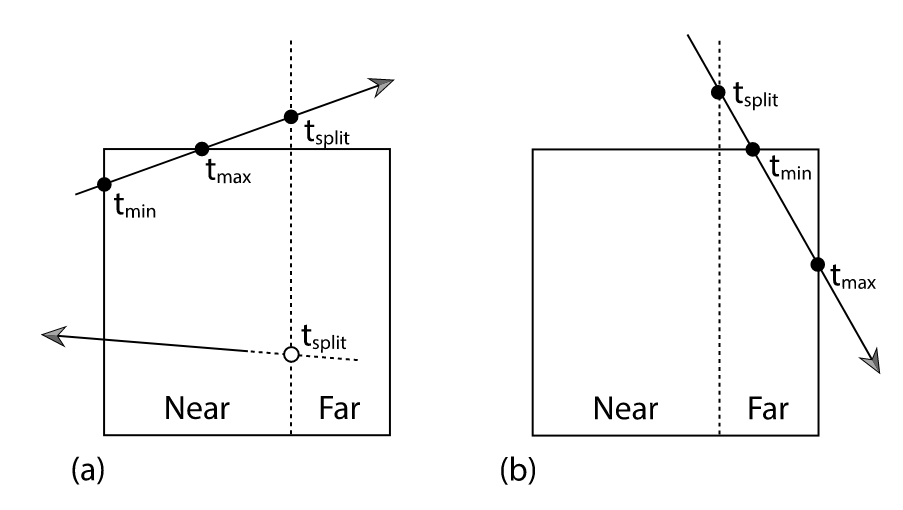
\includegraphics[width=10cm]{images/kdtree/traversal_case.png}
     \caption{Different scenarios prove the ray should not intersect both children.(a) The ray intersects the splitting plane at a point bigger than the $t_{max}$; hence we are sure it will not intersect the far child node. A negative sign denotes the bottom ray's direction away from the dividing plane. (b) In this case, the ray intersects the box at a point after the splitting plane, indicating that the  near child is avoided. \protect\cite{Pharr2016}}
        \label{fig:dice}
\end{figure}


\clearpage

\section{Performance Analysis}
In this chapter, we will analyze the different data structures used (BVH, LBVH, Kd-Tree) and how they perform against different scenes. We will pick up one data structure and tweak its different parameters and analyze how small changes in the parameter can affect the performance.


The following settings are used in the raytracer:
\begin{table}[ht] 
\centering 
{\footnotesize
\begin{tabular}{ P{2.5cm}||P{5cm}  P{5cm}}      % centered columns (3 columns) 
\hline \hline
\\
Property & Value & Note \\ [0.5ex]
\\
\hline \hline
\\
Machine & Intel(R) Core(TM) i7-8565U CPU @ 1.80GHz, RAM 16GB & -\\ [0.5ex] % inserts table heading 
\\
 \hline
 \\
Resolution & 640x480 & - \\
\\
 \hline
 \\
Programming language & C++ & - \\
\\ 
 \hline
 \\
Shader & Phong illumination & - \\
\\
 \hline
 \\
\#Cameras & 1 & - \\
\\
\#Lights & 1 & - \\
\\ 
 \hline
 \\
 Models extention& .obj& The extention that the raytracer supports \\
\\ 
 \hline
 \\
Anti-aliasing & 1 & Number of anti aliaising samples\\
\\ 
 \hline
 \\
Maximum number of leafs& 1 & The leaf node only containe one or less than one premitive\\
\\
\hline \hline
    \end{tabular}
}
\end{table}

\subsection{How tweaking the data structure parameters affect performance}
Before jumping to the next chapter "Tests and Performance Analysis", I would like to emphasize and explain how a small change in the parameter of building the tree can affect the performance significantly. 
\\
\noindent

Figure 20 shows two different constructed binary trees based on the same algorithm Kd-Tree and the same input scene, however by changing the maximum number of premitives in leaf node parameter, we can note that one tree is shorter than the other! How would this affect the performance? 
\\
\noindent

A deeper tree means more nodes which leads to more memory consumption. Moreover, if the splitting criteria are too bad this can lead to a long traversal time. On the other hand, a shallow tree can lead to fewer nodes but leaves that contain more primitives that will require a linear search (Brute force).    


\begin{figure}[H]	
     \centering
     \begin{subfigure}[b]{0.3\textwidth}
         \centering
         \captionsetup{justification=centering}
         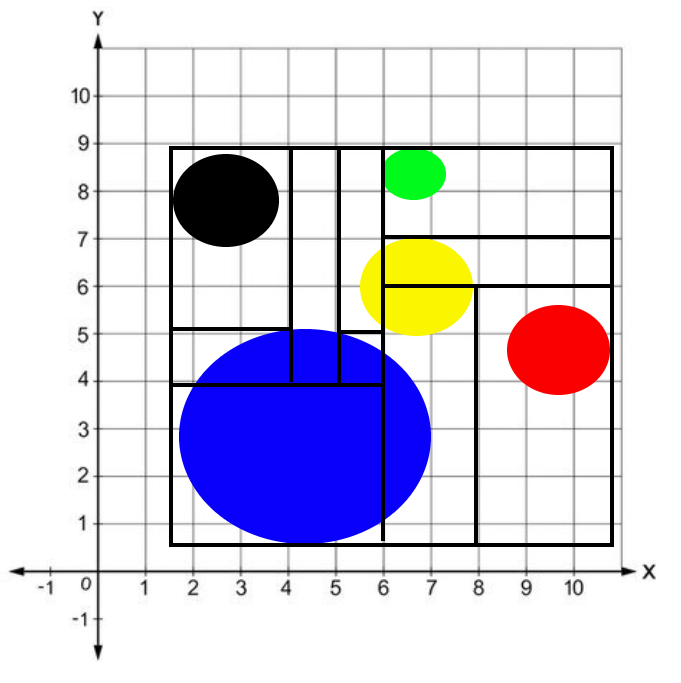
\includegraphics[width=\textwidth]{images/kdtree/visaul_scene_1.png}
         \caption{Kd-Tree generates regions (AABB) in a simple scene.}
         \label{fig:pi_4000}
     \end{subfigure}
     \hfill
     \begin{subfigure}[b]{0.6\textwidth}
         \centering
         \captionsetup{justification=centering}
         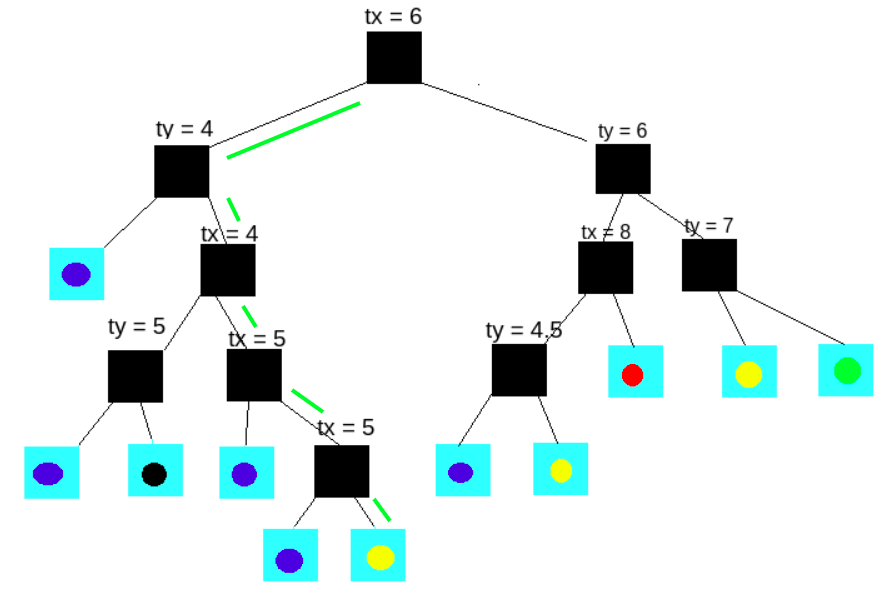
\includegraphics[width=\textwidth]{images/kdtree/visaul_tree_11_green.png}
         \caption{The resulting binary tree is based on the Kd-Tree algorithm with setting the maximum number of primitives in the leaf node parameter to 1.}
         \label{fig:pi_5000}
     \end{subfigure}
     \hfill
     \begin{subfigure}[b]{0.3\textwidth}
         \centering
         \captionsetup{justification=centering}
         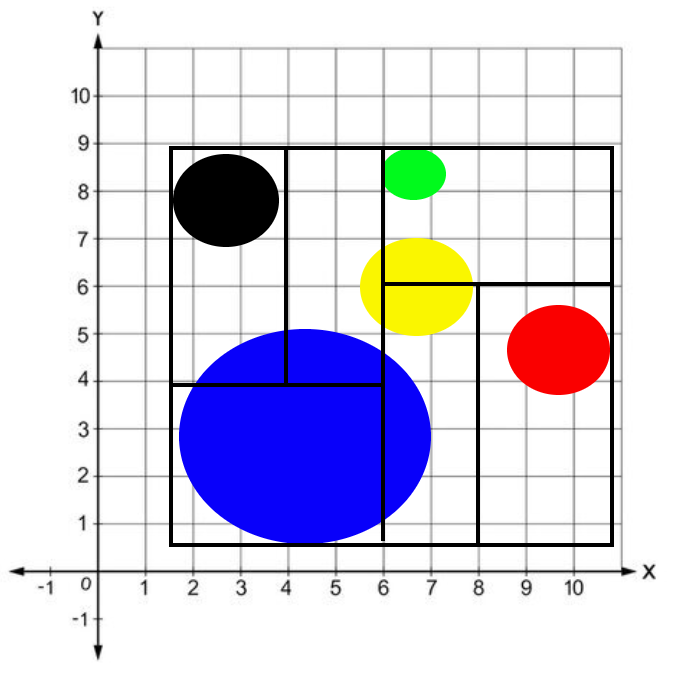
\includegraphics[width=\textwidth]{images/kdtree/visaul_scene_2.png}
         \caption{Kd-Tree generates regions (AABB) in a simple scene.}
         \label{fig:pi_5000}
     \end{subfigure}
     \hfill
     \begin{subfigure}[b]{0.6\textwidth}
         \centering
         \captionsetup{justification=centering}
         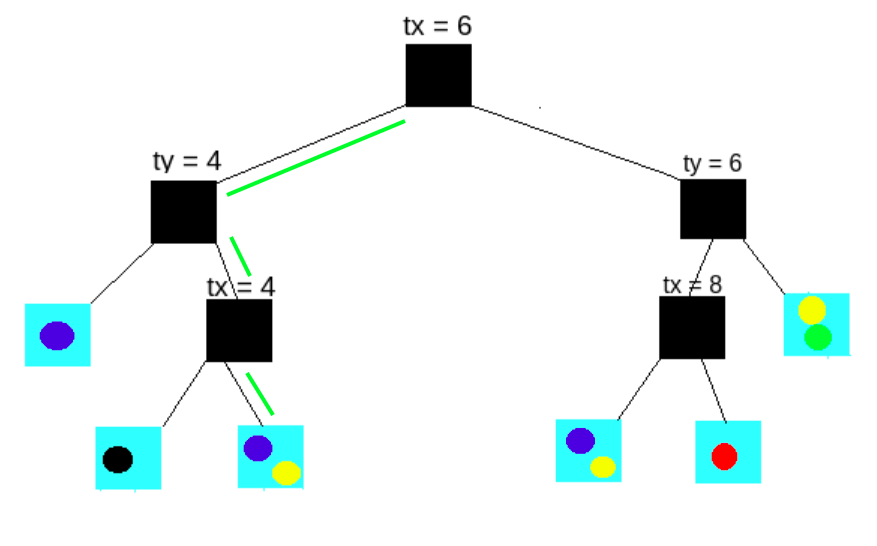
\includegraphics[width=\textwidth]{images/kdtree/visual_tree_2_green.png}
         \caption{The resulting binary tree is based on the Kd-Tree algorithm with setting the maximum number of primitives in the leaf node parameter to 2.
}
         \label{fig:pi_5000}
     \end{subfigure}
        \captionsetup{justification=centering,margin=2cm}
        \caption{Two different constructed kd-trees with the same implementation and scene but with different parameter.}
        \label{fig:three graphs}
\end{figure}

In order to demonstrate this in simple math. Assuming the time consumed to test the intersection with an AABB box will take $0.1ms$. We take the path demonstrated in the Figure in green that is been generated to find the intersection with the yellow sphere. (b) needs five AABB tests this will result in $0.5ms$ to find the intersection, unlike in (d) where only three AABB tests are needed resulting in $0.3ms$ to find the sphere. Obviously, the deeper tree has less performance! Nonetheless, we did not put the intersection cost of the spheres into consideration! In this example the sphere intersection cost is tiny but what if we replace the spheres with more complex models will the shallow tree still be better to use? In a shallow tree, the yellow sphere can be after the blue sphere in the list, hence one has to test the blue sphere first and then jump to the yellow. If the blue sphere (Model) in general has a high intersection cost let's say $0.3ms$. then this will be added to the shallow tree cost (d) to become $0.3ms + 0.3ms = 0.6ms$ which is larger than the long path in the deep tree (b). Even though the model is as simple as a triangle or sphere only, we need to remember that for the long list that contains a big number of primitives this will add a leaner complexity.
\\
\noindent

To investigate the concept of how changing the data structure parameters impacts the resulting tree which leads to different performance metrics, I have chosen one data structure Kd-Tree to verify this. In this experience, we will try changing two main parameters: The maximum number of primitives assigned to each leaf (maxPrims) and the Maximum depth of the tree (depth). For better testing, I have fixed the model which is the Stanford bunny. Moreover, other SAH parameters are fixed to focus only on the two parameters mentioned. 
\\
\noindent

By changing the maxPrims parameter and fixing the others we can note that the larger the value the less it takes to build the tree, for example when increasing maxPrims from  1 to 100, the build time increased by almost 2X. This is predictable as we discussed before, when the maxPrims parameter is big we stop the recursion of building the tree hence we stop creating more interior nodes as shown in the table the total number of nodes decreases by almost 418X consequently the tree depth becomes smaller. On the other hand, we note that rendering time increased by 1.2X. This is because for some leaf nodes now we have nodes with 100 primitives that the ray has to go through them linearly and test them until it finds the right primitive or even worse not find an intersection after going through 100 primitive intersections. This explains why the number of intersection tests shown in the table has increased by almost  61X. When the value is chosen between 10, this gave the best of both worlds, as the building and the rendering time are acceptable. 





\begin{table}[ht] 
\centering 
{\footnotesize
\begin{tabular}{ P{2.5cm} ||P{2.3cm}  P{2.3cm}  P{2.3cm} P{2.3cm}  P{2.3cm}}      % centered columns (3 columns) 
\hline\hline                                      %inserts double horizontal lines
\Includegraphics[height=1in]{images/stanford-bunny-black.png}
& \#Primitives  & \#Nodes & \#Primitives intersection tests & Build(s) & Rendering(s) \\ [0.5ex] % inserts table heading 
\hline
    \end{tabular}
}
\end{table}
\vspace{-2em}
\begin{table}[ht] 
\centering 
{\footnotesize
\begin{tabular}{ P{2.5cm} ||P{2.3cm}  P{2.3cm}  P{2.3cm} P{2.3cm}  P{2.3cm} }      % centered columns (3 columns) 
 \hline
\\
maxPrims = 1& 35, 947 & 418, 548 & 192, 171 &  5.214 s & 20.845 s\\
\\
maxPrims = 10& 35, 947 & 19, 229 & 1, 381, 296 & 2.033 s & 20.211 s\\
\\
maxPrims = 100& 35, 947 & 1, 461 & 11, 761, 329 & 2.865 s & 24.062 s\\
\\
\hline \hline
\\
depth = 5 & 35, 947 & 61 & 140, 964, 745 &  0.7 s & 37.762 s \\
\\
depth = 10& 35, 947 & 1, 435 & 10, 571, 611 & 1.239 s & 11.566 s\\
\\
depth = 28& 35, 947 & 44, 852 & 683, 669 & 1.757 s & 9.606 s\\
\\
depth = 100& 35, 947 & 44, 854 & 683, 669 & 1.871 s & 9.546 s\\
\\
\hline \hline
    \end{tabular}
}
\end{table}

The depth parameter has a different effect on the number of nodes where when the value changed from 5 to 10 the number of nodes increased by almost 24X which reduced the rendering time by almost 3X.  Even small values of the depth reduce the building time the rendering time which is usually the most critical stage in the raytracing pipeline is increased tremendously. Using the formula mentioned to set the depth dynamically depending on the scene, we end up with a value equal to 28 in this scene (Stanford bunny), this value increases the rendering time even more by almost 4X in comparison to depth equals to 5. Nevertheless increasing the depth more to 100 resulted in no performance gain as we reached a saturation point. Although I took the formula from the book PBRT for granted it seems that it delivers a decent result in this scene. 
\\
\noindent

What about tweaking both parameters to find the best result? In order to find the best combination of parameters for a random scene one can use one of the well known parameter optimization techniques such as  Grid Search, we will not cover this part in this report as I have used a simple manual method. 

\subsection{Investigating different data structures}
I have used different models with a diverse range of primitives for proper comparison. The models Stanford-bunny, Igea, Asian Dragon, and Happy Buddha used are taken from the following repository [commontest].
\\
\noindent

For all the three used data structures I have calculated a collection of useful mercies.  Since each data structure needs a pre-processing time to be constructed and built, build time in seconds corresponds to how many seconds each data structure took to be ready to be used for the rendering stage. Rendering time render is also important to be measured, as it indicates how long the overall rays took to travel through the scene. The number of intersection tests done for the primitives is also important as it explains how many intersection tests are done in the rendering phase, usually less number of intersection tests indicates better performance. The total number of nodes metric indicates the complexity of the constructed tree and how deep is it. 
\\
\noindent

The first metric to investigate is the building time. We can note that BVH is the fastest to build the tree and Kd-Tree takes 3X for the Stanford bunny and 6X for the Happy buddha, nonetheless, LBVH stays in between! BVH is the fastest because it uses simple splitting criteria which is the median of the AABB box, this is a cheap performance execution, moreover, it uses a simple tree representation and does not use a compact form. LBVH is almost 2X of the BVH, even though both are using the same binary tree the splitting criteria are different. LBVH has to map the center point of the 3D primitive to a Morton code, sort it by radix sort and then find a splitting point. These extra three stages add extra complexity to the building phase, hence LBVH takes more time than BVH for this implementation. Kd-Tree consumes so much time in the building phase since it uses the SAH algorithm for splitting nodes. As we explained already with an example the SAH method can be expensive to compute, especially for some edge cases where the splitting point can not be found and the algorithm tries the whole three different axes until it either find the best split or just split the AABB into halves. 
\\
\noindent

The second metric is the rendering time.  The first note is that both BVH and LBVH have similar performance at rendering, the reason is that both are using the same rendering algorithm. By adding both building and rendering time we can note that BVH spends less time than LBVH. So why are we using LBVH? LBVH is mostly beneficial on the construction time as the tree can be built on multi threads, however, I did not include this as it is intuitive multithreading will increase any algorithm performance. Kd-Tree on the other hand spends less time on the smaller models with few primitives as well as the ones with 1 million primitives. Adding both buildings the rendering time we note that Kd-Tree consumes much more time than the other data structures. 
\\
\noindent

Looking at the number of nodes and the number of intersections with primitives we can see that kd-Tree is a clear winner, and this explains why Kd-Tree spends less time on rendering than BVH and LBVH. Note that number of nodes in the Kd-Tree is less due to two reasons. The first reason is that we are using the equation mentioned to calculate the maximum depth for the tree which will restrict its recursions and the nuumber of splitting, unlike BVH and LBVH where both do not care about depth in my implementation.  The second reason is that we used SAH for splitting which looks for the tradeoff between the cost of splitting or just creating a leaf node and stopping. 
\\
\noindent

\begin{table}[ht] 
\centering 
{\footnotesize
\begin{tabular}{ P{2.5cm}||P{2.5cm}P{2.5cm} P{2.5cm} P{2.5cm}  }      % centered columns (3 columns) 
\hline\hline                                      %inserts double horizontal lines
& Bunny  & Igea & Asian Dragon & Happy Buddha \\ [0.5ex] % inserts table heading 
\hline\hline 

&
\Includegraphics[height=1in]{images/stanford-bunny-black.png}& \Includegraphics[height=1in]{images/igea-black.png} & \Includegraphics[height=1in]{images/xyzrgb_dragon.png} & \Includegraphics[height=1in]{images/happy-black.png} \\

\hline \hline
\\
\#Primitives & 35, 947  & 134, 345 & 539, 205 & 1, 078, 410 \\ [0.5ex] % inserts table heading 
\\
\hline \hline

\\
BVH build(s)& 0.849 s& 2.739 s & 21.105 s & 34.687 s \\
\\
LBVH build(s)& 1.272 s& 4.401 s & 45.98 s & 58.234 s \\
\\
Kd-Tree build(s)& 2.346 s& 30.075 s & 120.078 s & 211.078 s \\
\\
\hline \hline
\\
BVH render(s)& 17.707 s& 13.986 s & 41.588 s & 51.516 s \\
\\
LBVH render(s)& 11.512 s& 13.796 s & 40.744 s & 51.14 s \\
\\
Kd-Tree render(s)& 9.405 s& 12.111 s & 45.292 s & 34.292 s \\
\\
\hline \hline
\\
BVH \#int. tests & 139, 926 & 365, 715  & 2, 429, 951  & 3, 279, 593  \\
\\
LBVH \#int. tests & 93, 641 & 365, 712  & 2, 429, 942  & 3, 279, 593  \\
\\
Kd-Tree \#int. tests & 128, 943 & 74, 516  & 483, 710  & 943, 201  \\
\\
\hline \hline
\\
BVH \#nodes & 71, 893 & 268, 689  & 1, 078, 409  & 2, 156, 819  \\
\\
LBVH \#nodes & 71, 889 & 268, 669  & 1, 077, 768  & 2, 156, 352  \\
\\
Kd-Tree \#nodes & 418, 661 & 2, 830, 597  & 415, 406  & 375, 243  \\
\\
\hline \hline

    \end{tabular}
}
\end{table}

Note that even though the average performance is correlated with the number of primitives in the scene, however, there are some scenarios where the performance is not behaving as expected. For example, looking at the Kd-Tree number of nodes can spike up, this is because not only the number of primitives important to choosing the right data structure but other perspectives related to the scene can affect the performance not only the number of primitives.  The next tests try to cover some of them.

\clearpage

\section{Conclusion}
\cite{pharr2016physically}
\cite{burley2018design}
\cite{stanfordlucy}

\clearpage

\bibliographystyle{apacite}
\bibliography{References}

\end{document}
